\chapter{Air Track}

\section*{Objectives}

\begin{enumerate}
\itemsep0em
\item To study motion in one dimension in a near-frictionless set-up.
\item To attempt to verify Newton's three laws of motion.
\end{enumerate}


\section*{Introduction}

Newton's second law famously relates the externally applied force on an object to its acceleration,
\begin{equation}
    \vb{a} = \left(\frac{1}{m}\right) \vb{F}.
    \label{airtrack-newtonslaw}
\end{equation}

\begin{question}
 \textbf{Question:} You are probably a little uncomfortable about the way Equation~(\ref{airtrack-newtonslaw}) has been written. Can you explain why this way is, in some sense, superior to the common $\vb{F}=m\vb{a}$?
\end{question}

 From the above equations, it should be clear that if a body is given an initial velocity, and no external force is applied to it, it should continue to move at that velocity. In other words, its position should vary linearly with time.
 
 However, this clearly contradicts our everyday experience. Imagine placing your book on the table and giving it an initial velocity by pushing it and letting go: the book will, at best, move a little and come to rest. This does not, of course, contradict Newton's second law. The surface applies a force to the object that opposes its motion. Such ``frictional'' forces are notoriously difficult to take into account, and so if we want to study simple one dimensional systems, it would be helpful to minimise them as far as possible. However, if you imagine an object in outer space, it is not difficult to see that giving it a push will cause it to move at a constant velocity.
 
 It is not possible for us to conduct this experiment in outer space. However, what essentially distinguishes the environment in outer space from the table-top is the presence of friction. A device that almost eliminates friction if the air track, which simulates a low-friction environment by creating a ``cushion'' of air on which an object (called a ``rider'') may float. 
 
\begin{figure}[!htb]
     \centering
     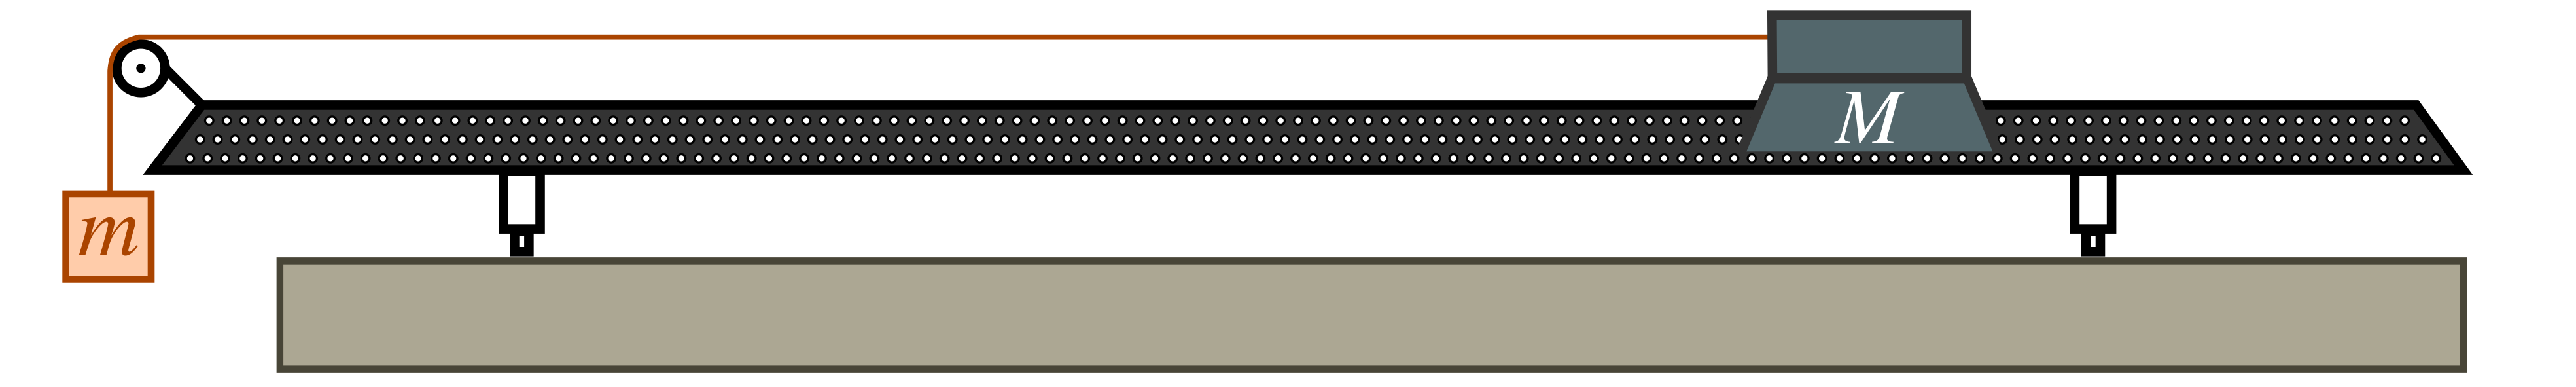
\includegraphics[width=0.9\textwidth]{figs/airtrack/airtrack-setup.png}
     \caption{Schematic of the set-up. A rider of mass $M$ floats on the track, and is connected to a mass $m$ through a pulley and an inextensible string. As the mass $m$ is allowed to fall, the rider experiences a constant acceleration. }
     \label{fig:airtrack}
 \end{figure}

\section*{Theory}

\subsection*{Uniformly accelerated motion}

\begin{question}
    \textbf{Question:} Consider an object of mass $m$ acted on by a constant force $F_0$. Show, by integrating Newton's second law, that the object's velocity and position vary as
    \begin{equation}
    \begin{aligned}
     v(t) &= v(0) + \left(\frac{F_0}{m}\right) t,\\
     x(t) &= x(0) + v(0) t + \frac{1}{2} \left(\frac{F_0}{m}\right) t^2.
    \end{aligned}
    \end{equation}
\end{question}

To test the above equations, we impose a constant force on the rider. Consider setting the air track up as shown in Figure~(\ref{fig:airtrack}). Connect a mass $m$ to the rider (of mass $M$) with an inextensible string. When the mass $m$ is released, the only horizontal force on the rider comes from the tension $T$ on the string, and so 
\begin{equation}
M a = T.
\end{equation}

\begin{question}
\textbf{Question:} Can you argue that the two blocks must accelerate at the same rate $a$? What assumptions do you need to make for this?
\end{question}

The hanging mass $m$ feels both gravity (downwards) and tension $T$ (upwards), so that
\begin{equation}
m a = mg - T.
\end{equation}

\begin{question}
\textbf{Question:} Show that by measuring the acceleration of the rider, one can measure the acceleration due to gravity $g$, since
\begin{equation}
g = a \left(\frac{M+m}{m}\right).
\end{equation}
\end{question}

\subsection*{Conservation of momentum}

When such a low-friction environment ensures that (almost) no external forces are acting on the object, Newton's second law tells us that the quantity $m\times v$ is a constant. When we have a single object, this just tells us that -- when there are no external forces acting on the object -- its momentum stays constant. If, in addition, the mass of the object is constant, this is just a statement that the velocity remains constant.

Such ``momentum conservation'' applies to a single object, but it is a lot more interesting to look at a situation with at least two interacting objects. Consider two objects moving at constant velocities (say $v_1$ and $v_2$) which collide. From Newton's third law, the force of the first on the second (say, $F_{12}$) is equal and opposite to the force of the second on the first ($F_{21}$). Thus,
\begin{equation}
F_{12} = - F_{21}.
\end{equation}

If we consider that the forces act over a small time interval $\Delta t$, it follows that the impulses experienced by the two objects are also equal in magnitude and opposite in direction, i.e.\ 
\begin{equation}
\begin{aligned}
 F_{12} \Delta t &= - F_{21} \Delta t,\\
 m_1 \Delta v_1 &= - m_2 \Delta v_2,
 \end{aligned}
\end{equation}
where in the last case we have simply used the definition of the acceleration. Thus, we can see that the change in momentum of each mass is equal in magnitude, but opposite in sign: momentum is \textsl{transferred} from one object to the other.

\begin{question}
\textbf{Question:} In the above case, show that the velocities before and after the collision are related by:
\begin{equation}
m_1 v_1^\text{before} + m_2 v_2^\text{before} = m_1 v_1^\text{after} + m_2 v_2^\text{after}
\end{equation}
\end{question}

\subsection*{Elastic and inelastic collisions}

It may have struck you that in the earlier case we seemed to imply that after the collision the objects moved away at different velocities, and thus remained \textsl{distinct} (consider two billiard balls colliding). However, from real world experience you have often seen another case: collisions where the two objects ``stick'' together, and thus move at together at the same velocity after the collision (consider two lumps of clay thrown at each other). Consider both these cases: since we could engineer it such that the objects (billiard balls or lumps of clay) have the same masses and the same velocities, and since we know that the results after the collisions are clearly different, there must be some way to distinguish between them.

You will show, in your course on \textsl{Classical Mechanics}, that the distinction between such collisions is to do with another conserved quantity: energy. In particular, the kinetic energy (or the energy that an object possesses by virtue of its motion) is given by \begin{equation}
\text{KE} = \frac{1}{2} m v^2.
\end{equation}

We can use the kinetic energy to classify collisions into two types:
\begin{enumerate}
 \item \textbf{Perfectly elastic} collisions in which both momentum and kinetic energy are conserved. In other words, if two masses $m_1$ and $m_2$ and velocities $v_1$ and $v_2$ collide elastically and move away with velocities $v'_1$ and $v'_2$, then
 \begin{equation}
 \begin{aligned}
     m_1 v_1 + m_2 v_2 &= m_1 v'_1 + m_2 v'_2,\\
    \frac{1}{2}m_1 v_1^2 + \frac{1}{2} m_2 v_2^2 &= \frac{1}{2}m_1 {v'_1}^2 + \frac{1}{2} m_2 {v'_2}^2.
 \end{aligned}
 \end{equation}
 \item  \textbf{Perfectly inelastic} collisions in which momentum is conserved, but kinetic energy is not conserved. In other words, if the masses stick together to form a mass of $m_1 + m_2$ moving at some velocity $V$, then
 \begin{equation}
 \begin{aligned}
     m_1 v_1 + m_2 v_2 &= (m_1 + m_2)V,\\
    \frac{1}{2}m_1 v_1^2 + \frac{1}{2} m_2 v_2^2 &\neq \frac{1}{2}(m_1+m_2) V^2.
 \end{aligned}
 \end{equation}
\end{enumerate}

\begin{imp}
It is important to realise that while \textsl{kinetic} energy is not conserved, this does not mean \textsl{energy} is not conserved. Since energy can take different forms, some of the initial kinetic energy may go into deforming the objects, or producing heat. In general, most collisions are inelastic (though not \textsl{perfectly} inelastic), and some energy is always lost to the environment.
\end{imp}

\begin{question}
 \textbf{Question:} Perfectly elastic collisions generally only occur at the atomic scales. The example of two billiard balls is not a perfectly elastic collision. Where do you think the lost kinetic energy goes?
 
 \textbf{Question:} Show that in perfectly inelastic collisions above, the ``loss'' in kinetic energy is can be written as 
 \begin{equation}
     \text{Loss in KE} = \frac{1}{2} \mu \, (v_2 - v_1)^2.
 \end{equation}
 Where you need to determine $\mu$ (called the \textsl{reduced mass} of the body). What do you think this means? 
\textbf{Hint:} Imagine placing yourself in the reference frame of the centre of mass of the two objects.
\end{question}




\section*{Experimental Setup}

\subsection*{Apparatus}

\begin{enumerate}
\itemsep0em
\item A 2 metre-long air track
\item A blower to pump air through the track
\item Assorted accessories including riders and their attachments (shown in Figure~(\ref{fig:airtrack-accessories}))
\item Two photogates and associated their cables (\textsl{Vernier} or \textsl{Indosaw})
\item Retort stands to position the photogates
\end{enumerate}


\subsection*{Description}

\begin{figure}[!htb]
    \centering
    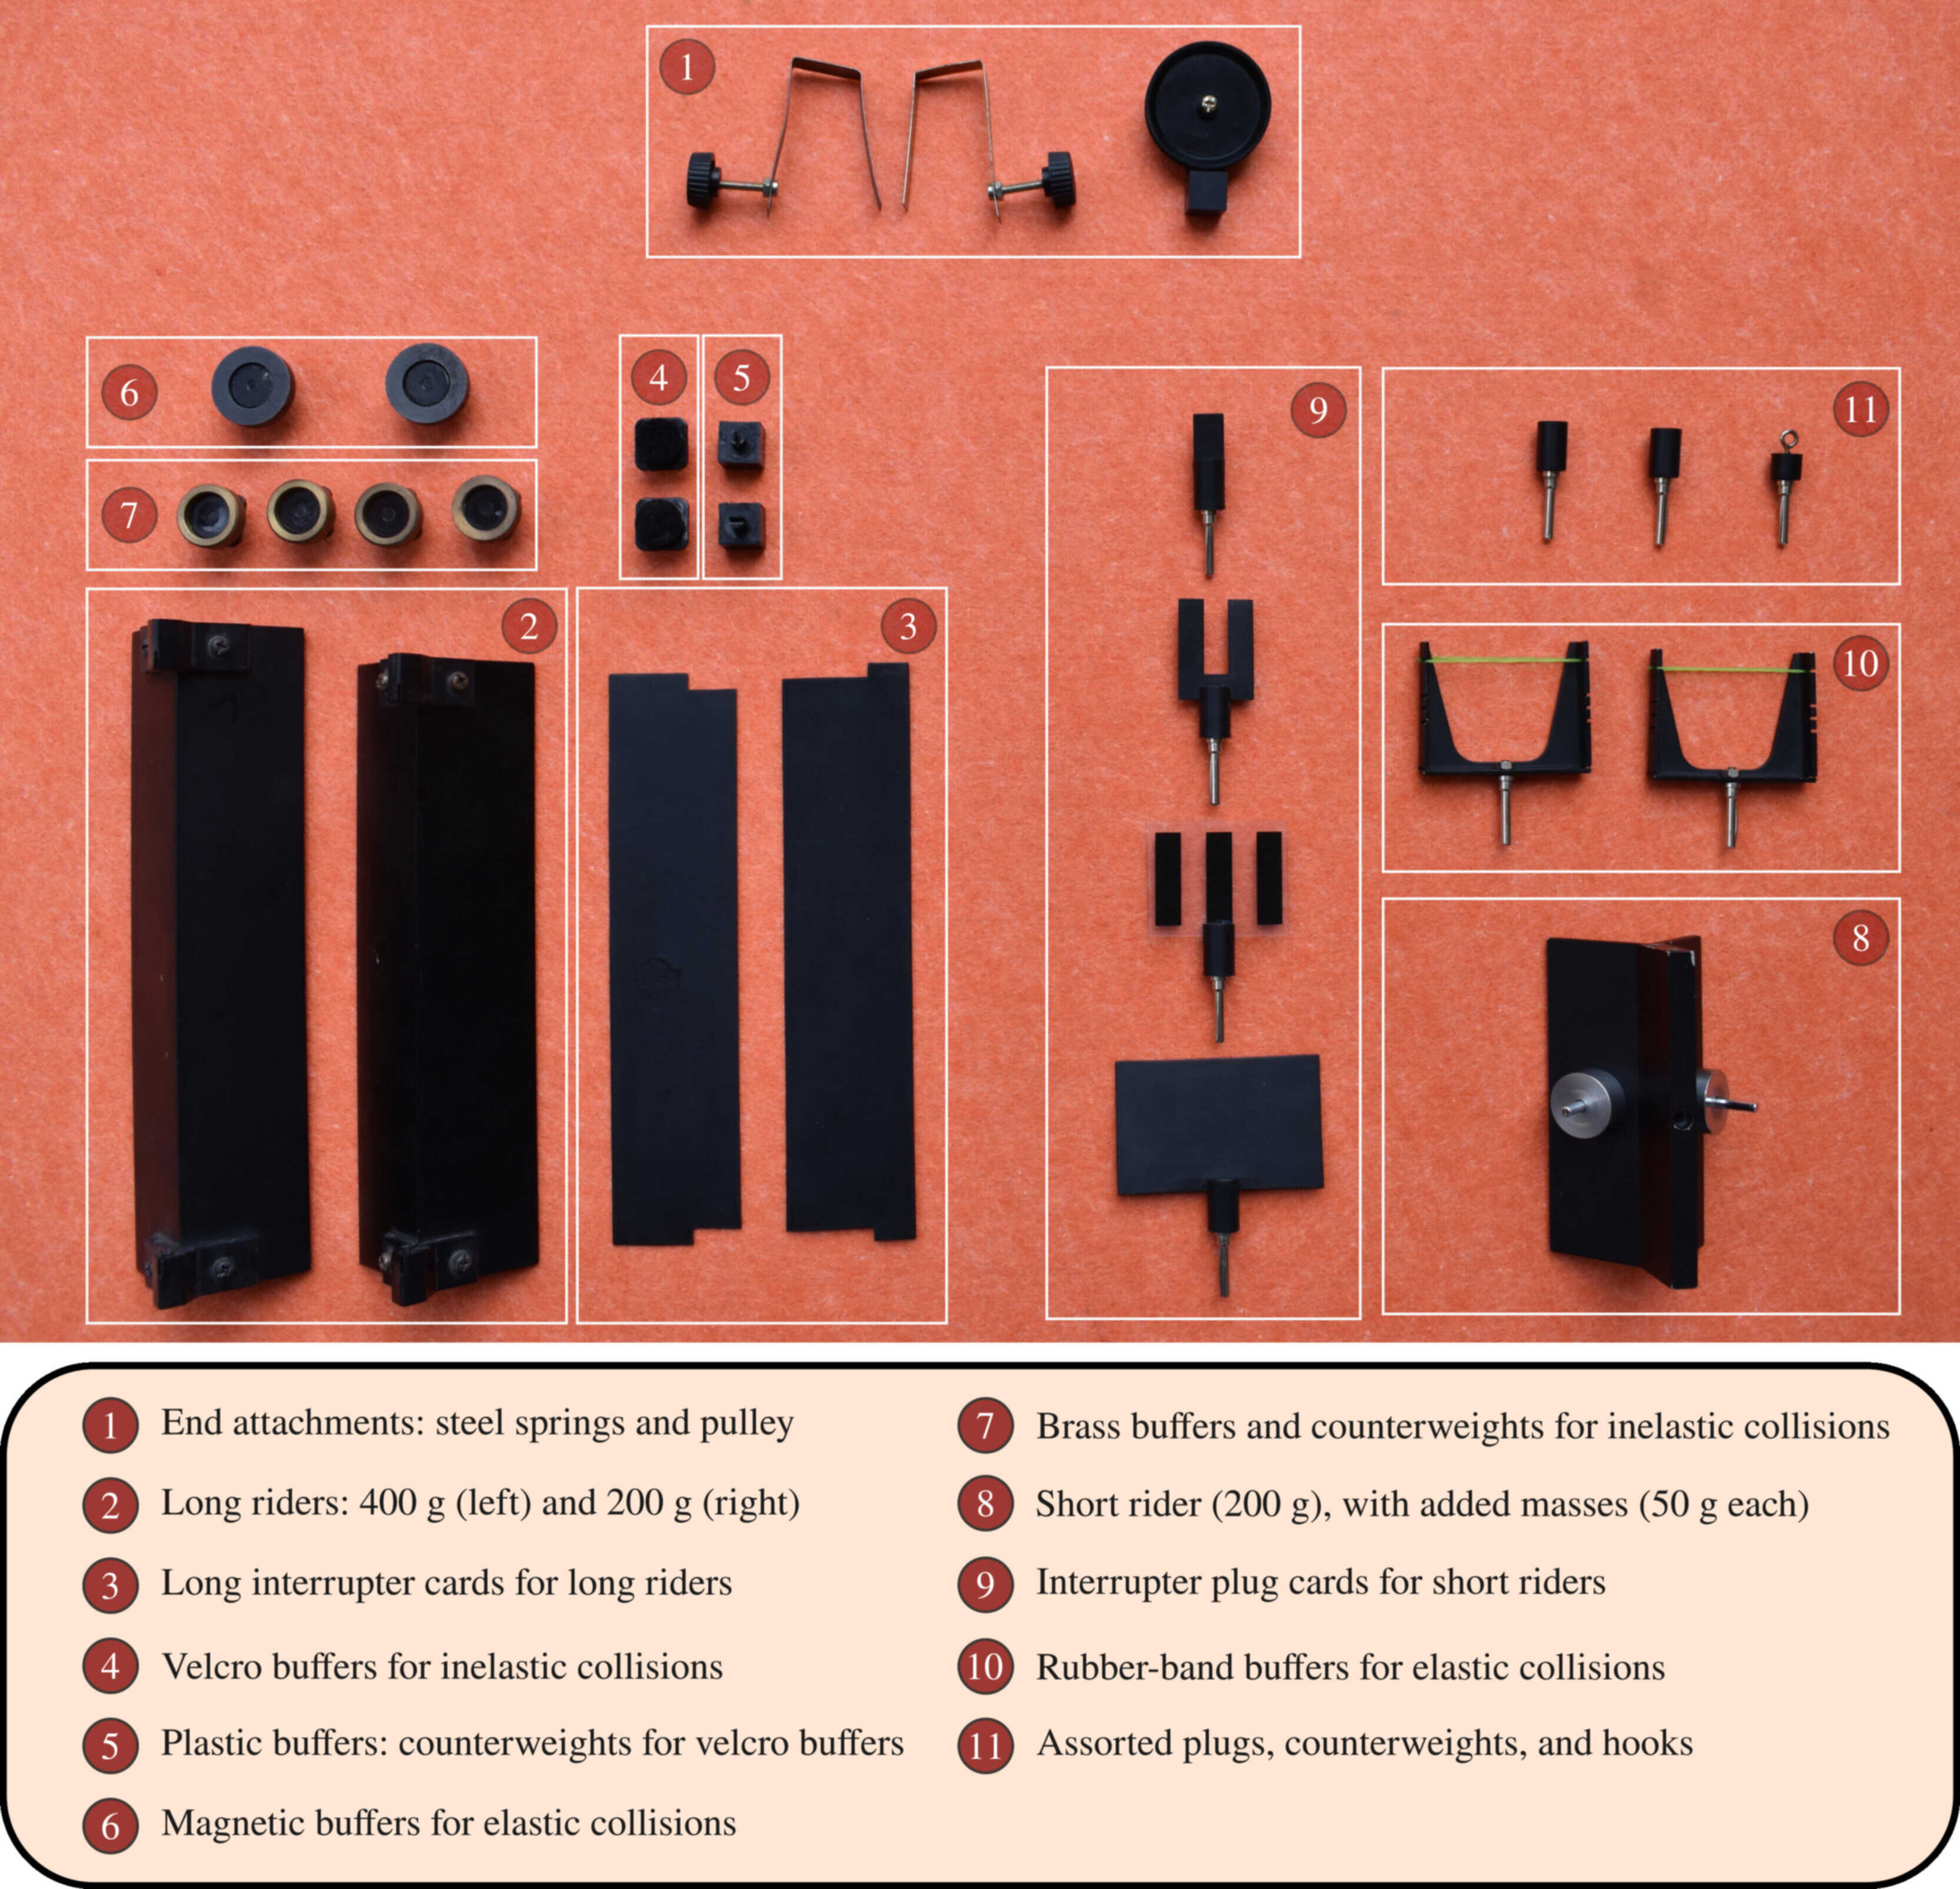
\includegraphics[width=\textwidth]{figs/airtrack/airtrack-accessories.jpg}
    \caption{Accessories for the air track. The end attachments are placed at either end of the track. The remaining accessories are placed on one of the two different types of riders, long or short. The long riders come in two types: the heavier 400 g rider is slightly longer than the 200 g rider. On the left are all the attachments for the long riders, and on the right are all the attachments for the short riders.}
    \label{fig:airtrack-accessories}
\end{figure}

\subsubsection*{The air track}

The air track, as explained, can be used as a low-friction environment for kinematics experiments. Compressed air is injected into the cavity beneath the track. Since this cavity is sealed, the air can only escape through the small holes on the track. This provides a force strong enough to lift the riders, drastically lowering the contact friction.

Connect the hose from the blower to the air track and turn it on. The speed of the blower (and thus the pressure on the rider) can be controlled by the knob on the blower.

The first step is to level the track, which you will do with a spirit level by adjusting its legs. A good way to test if the track is levelled and the pressure is sufficient is simply to place one of the riders on it and observe its behaviour. If the rider floats gently above the track and shows no preference for the right or left end, your air track is ready to use. 

\begin{tip}
Do not be tempted to keep the blower at maximum: too much pressure will cause more air to escape near the inlet than elsewhere, which will cause turbulence and destabilise experiments. On the other hand, using the bare minimum pressure requires you to be sure that the track is completely free of scratches or dirt on its surface. Try to find a middle ground before you start.
\end{tip}

\subsubsection*{End attachments}

The steel springs and pulley given with the set-up may be attached to the ends of the air track. The springs can be used to launch the riders, or to allow them to bounce back nearly elastically. The pulley may be placed on one end to change the direction of an applied force from vertical to horizontal.

\subsubsection*{Riders}

\begin{figure}[!htb]
    \centering
    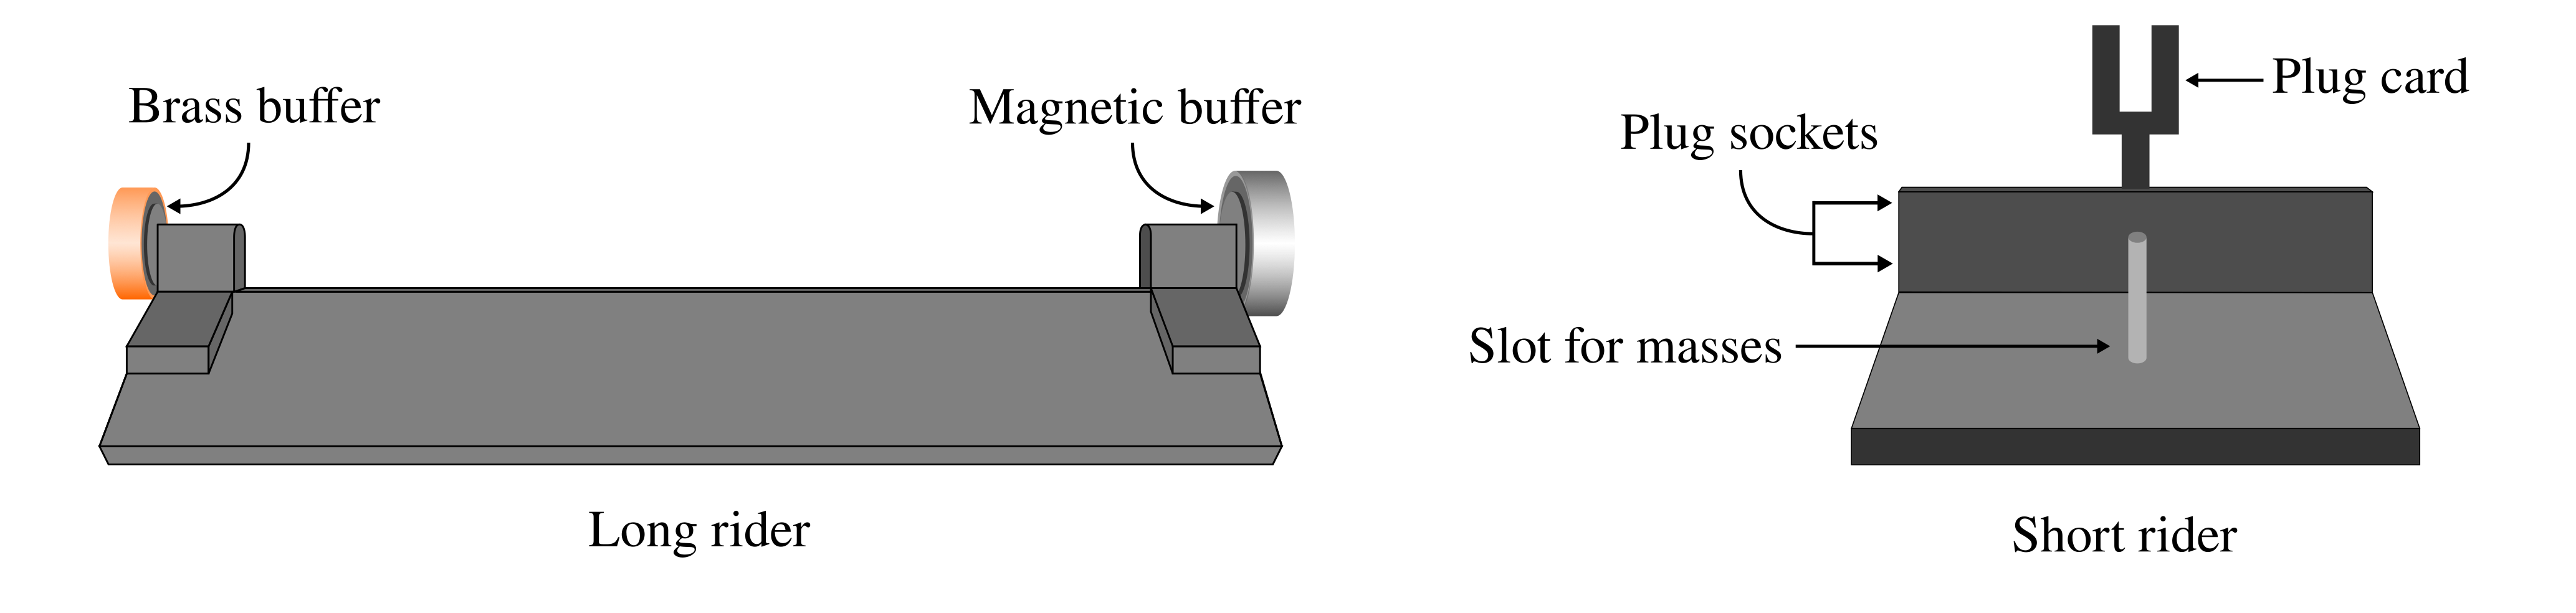
\includegraphics[width=\textwidth]{figs/airtrack/airtack-riders.png}
    \caption{Two sizes of riders, long and short. Short riders weigh roughly 200 g, and have slots on either side on which masses may be placed to increase the rider's weight. Two types of long riders are provided, one weighing 200 g and the other 400 g. }
    \label{fig:airtrack-riders}
\end{figure}

The air track has three different types of riders, on top of which the different interrupter cards and prongs may be added when working with the photogates. The riders can be distinguished by their mass and size:

\begin{enumerate}
    \item \textbf{Short rider} ($\sim 200$ g) with attachments on either side to add masses. (Make sure that the masses are added symmetrically on both sides.) The hole on the top may be used to attach the photogate flags to the rider.
    
    \item \textbf{Long rider} ($\sim 200$ g) along the top of which the short interrupter cards may be slotted.
    
    \item \textbf{Long rider} ($\sim 400$ g) along the top of which the longer interrupter cards may be slotted.
\end{enumerate}

\subsubsection*{Buffers and counterweights}

The riders have two holes on their edges, at different heights, to which different buffers may be attached. 

\begin{imp}
Whenever a buffer is added on one side, a counter-weight or plug must be added on the other side, to avoid the air track leaning to one end. If this happens, there will be an unbalanced horizontal force which will make the rider move in the direction it leans.
\end{imp}

\begin{enumerate}
    \item \textbf{Rubber-band bumpers} may be connected to the riders to simulate nearly elastic collisions. In order to do this, the bumpers will each need to be aligned at 45$^\circ$ to the riders in opposite directions, such that the elastic bands are perpendicular to each other, ensuring that they have plenty of room to stretch.
    
    \item \textbf{Magnetic buffers} may also be connected for nearly elastic collisions. As they act over a distance, no physical contact is made, and thus no energy can be lost to heat or sound.
    
    \item \textbf{Brass buffers} may be used as counterweights when the magnetic buffers are used for elastic collisions, but can also be used for inelastic collisions, as they lose energy as heat and sound when they collide. In this case, take care to add the magnets on the other side, as counterweights.
    
    \item \textbf{Velcro buffers} may be used to simulate perfectly inelastic collisions, as they will force the vehicles to stick together after impact. When these are used, appropriately sized plastic buffers should be used as counterweights.
    
    \item \textbf{Plastic buffers} are generally used as counterweights, but are suitable for inelastic collisions as well, provided the Velcro buffers are used as counterweights.
\end{enumerate}


\subsubsection*{The photogates}

\begin{figure}[!htb]
    \centering
    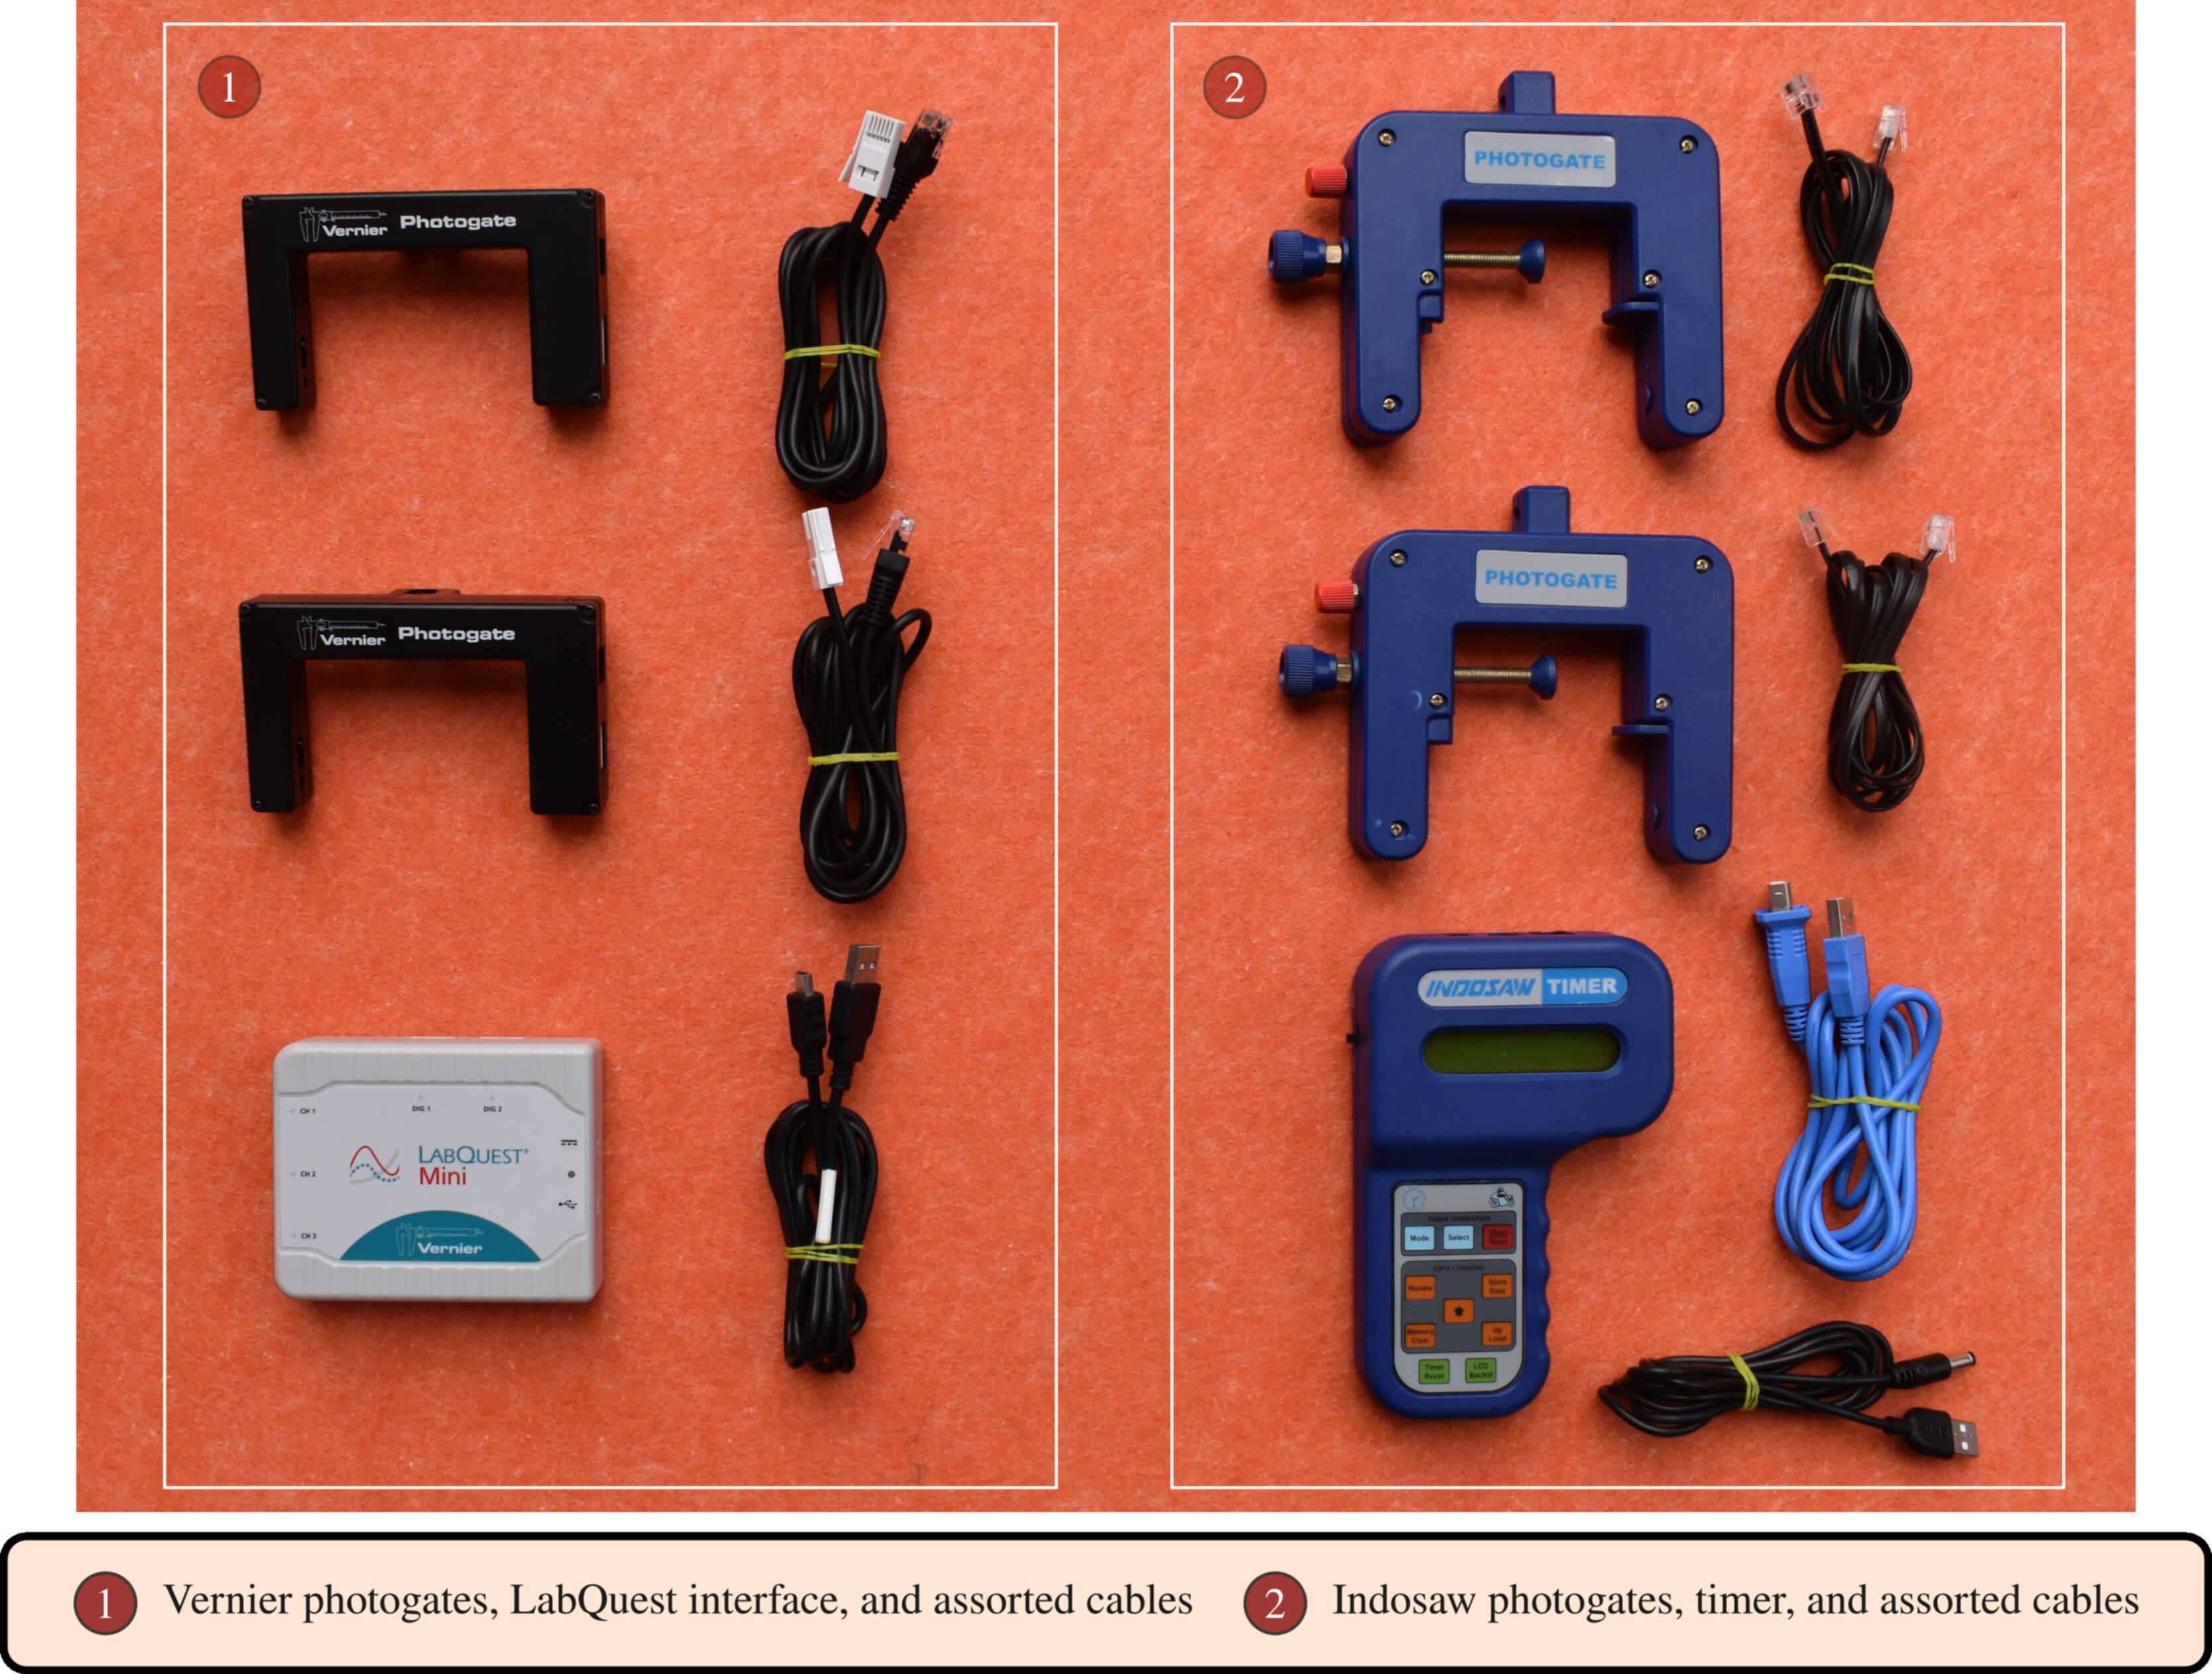
\includegraphics[width=\textwidth]{figs/airtrack/airtrack-photogates.jpg}
    \caption{Available photogates. The Vernier photogates (left) are controlled through the LabQuest interface which connects to a computer, while the Indosaw setup (right) has its own timer.}
    \label{fig:airtrack-photogates}
\end{figure}

Photogates allow for extremely accurate timing of events within physics experiments. They work by changing the state of their output signal whenever an object comes in between their infrared sensors, which allows us to measure the time interval $\Delta t$ the object takes to pass through the gate. If the object is sufficiently small -- and has a known length $\Delta x$ -- then we can find a good approximation of its instantaneous velocity,
\begin{equation}
    v \approx \frac{\Delta x}{\Delta t}.
\end{equation}
If the instantaneous acceleration is required, an interrupter with two prongs may be used. By measuring the change in velocity between these prongs $\Delta v$ and the change in time $\Delta t$, the instantaneous acceleration may be approximated as
\begin{equation}
    a \approx \frac{\Delta v}{\Delta t}.
\end{equation}

You have two types of photogates, \textsl{Vernier} and \textsl{Indosaw}, shown in Figure~(\ref{fig:airtrack-photogates}). The Vernier photogates will be used with the \textsl{LabQuest} interface and its data can be collected and analysed using the \textsl{LoggerPro 3} software. Each gate has an input port so multiple gates can be connected in a ``daisy-chain'' configuration. With the \textsl{LabQuest} interface and Vernier gates, up to four gates can connect to a single interface channel. The Vernier photogate also has a laser gate mode, which requires the addition of a common pen laser, which is directed into the laser port. The laser may be some distance from the gate, so that you can measure the speed of larger objects.


\begin{tip}
    Tutorials for the Vernier photogates can be found online,\footnote{\nolinkurl{https://www.vernier.com/training/videos/play/?video=201}} as can the manual. Make sure you go through them before collecting data to avoid making common mistakes.
\end{tip}

\subsection*{Precautions}
\begin{itemize}
\itemsep0em
\item \textbf{The air track must be level}! First use a spirit level to level the track roughly, then place a rider at different points on the track and adjust the legs until it shows no preference for the left or right end of the track.

\item Make sure the track's surface is clean, and none of the holes are plugged by dirt.

\item Ensure that the rider never tilts towards one direction. If this happens, you have either placed the weights asymmetrically or forgotten the counterweights.

\item If the rider wobbles, the air pressure is too high.

\item The collisions need to be as gentle as possible. A large source of uncertainty is the transfer of energy to the air track and table.
\end{itemize}

\begin{imp}
\textbf{Inherent errors:}
The riders are supported by a thin film of air approximately 0.01 cm thick. This film exerts a viscous drag on moving surfaces which should -- in theory -- cause the rider to gradually slow down until it comes to rest. However, practically, the rider oscillates around a position midway between the air holes. An air track with a practically infinite number of air holes would eliminate this problem, but this is not reasonable. Increasing the thickness of the film of air would reduce the coefficient of friction, but this would be at the expense of the rider's stability. Another potential source of error is the straightness of the air track. While an ideal air track should not sag, our tube is still heavy enough to sag slightly under the force of gravity. 
\end{imp}


\section*{Procedure}
\subsection*{Part A}

In the first part of this experiment, you will attempt to verify Newton's first law, showing that when an object experiences no external force, it travels in uniform rectilinear motion.

\begin{enumerate}
    \item Set up the metal springs at either end of the air track. Placing the rider at one end of the track, gently push it against the spring and let go.
    
    \item Measure the velocity of the rider using the photogates at two different points in its trajectory, and measure its velocity at both points.
    
    \item Repeat this for different initial velocities.
\end{enumerate}

\begin{question}
 \textbf{Question:} Assuming the steel spring to be ideal, show that the velocity of the rider is directly proportional to its initial displacement of the spring.
\end{question}

\subsection*{Part B}

Next, you will attempt to verify Newton's second law showing that under a constant force, the riders move with a constant acceleration.

\begin{enumerate}
    \item Remove one of the steel springs and connect the pulley. Pass a long string across the pulley and connect it to the rider at one end, and a slotted mass at the other, as shown in Figure~(\ref{fig:airtrack}).
    
    \item With the rider at one end, drop different masses and measure the change in velocity between two points along the riders trajectory to measure the acceleration.
    
    \item Plot a graph to calculate the acceleration due to gravity.
\end{enumerate}

\subsection*{Part C}

Finally, you will attempt to verify Newton's third law by colliding different riders together and measuring the momentum immediately before and after the collision.

\begin{enumerate}
    \item Put the steel spring back at the end of the air track, and attach two buffers (and counterweights) to the riders to simulate elastic collisions.
    
    \item Place the photogates such that the initial and final velocities of both the riders may be determined.
    
    \item Collide the two riders elastically using different initial conditions. If you need to launch the riders at the same speeds, use the steel springs as done in \textbf{Part A}.
    
    \item Replace the elastic buffers and with brass or Velcro buffers (and counterweights) to simulate inelastic collisions.
    
    \item In each case, calculate the loss in kinetic energy and compare it to the theoretically expected value.
\end{enumerate}